%!TEX root = ../../main.tex

\documentclass[../../main.tex]{subfiles}

\begin{document}
	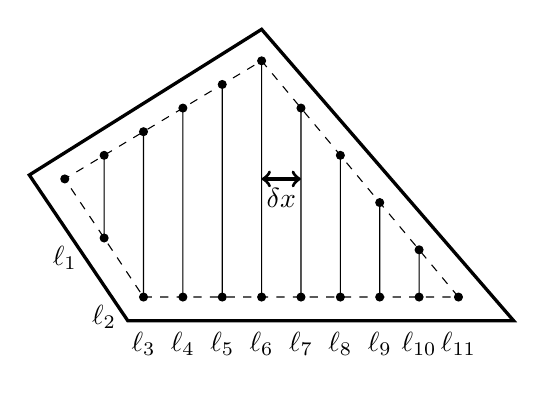
\begin{tikzpicture}[scale=1]

		\draw[dashed] (1,0)--(5,0)--(2.5,3)--(0,1.5)--cycle;
		\draw[very thick] (0.8,-0.3)--(5.7,-0.3)--(2.5,3.4)--(-0.45,1.55)--cycle;

		\draw[fill] (0,1.5) node [yshift=-1cm] {$\ell_1$}circle [radius=0.05];
		\draw[fill, -] (0.5,0.75) node  [yshift=-1cm]{$\ell_2$} circle [radius=0.05]--(0.5,1.8) node{} circle [radius=0.05];
		\draw[fill, -] (1.0,0.0) node [yshift=-0.6cm]{$\ell_3$} circle [radius=0.05]--(1,2.1) node {} circle [radius=0.05];
		\draw[fill, -] (1.5,0.0) node [yshift=-0.6cm]{$\ell_4$} circle [radius=0.05]--(1.5,2.4) node{} circle [radius=0.05];
		\draw[fill, -] (2.0,0.0) node [yshift=-0.6cm]{$\ell_5$} circle [radius=0.05]--(2.0,2.7) node{} circle [radius=0.05];
		\draw[fill, -] (2.5,0.0) node [yshift=-0.6cm]{$\ell_6$} circle [radius=0.05]--(2.5,3.0) node{} circle [radius=0.05];
		\draw[fill, -] (3.0,0.0) node [yshift=-0.6cm]{$\ell_7$} circle [radius=0.05]--(3.0,2.4) node{} circle [radius=0.05];
		\draw[fill, -] (3.5,0.0) node [yshift=-0.6cm]{$\ell_8$} circle [radius=0.05]--(3.5,1.8) node{} circle [radius=0.05];
		\draw[fill, -] (4.0,0.0) node [yshift=-0.6cm]{$\ell_9$} circle [radius=0.05]--(4.0,1.2) node{} circle [radius=0.05];
		\draw[fill, -] (4.5,0.0) node [yshift=-0.6cm]{$\ell_{10}$} circle [radius=0.05]--(4.5,0.6) node {} circle [radius=0.05];
		\draw[fill, -] (5.0,0.0) node [yshift=-0.6cm]{$\ell_{11}$} circle [radius=0.05]--(5.0,0.0) node {} circle [radius=0.05];

		\draw[very thick, <->] (2.5,1.5)--(3,1.5);

		\node [below] at (2.75,1.5) {$\delta x$};

	\end{tikzpicture}
\end{document}